\documentclass[11pt]{article}
\usepackage[margin=1in]{geometry}
\usepackage{amsmath,amssymb,booktabs,graphicx,hyperref}
\hypersetup{colorlinks=true,linkcolor=blue,urlcolor=blue,citecolor=blue}
\title{Learning to Restore Operational Histories from Executable Temporal Worlds}
\author{Author details pending final review}
\date{Development manuscript: 15 October 2026}
\begin{document}
\maketitle
\begin{center}\fbox{\parbox{.9\linewidth}{\textbf{Internal development draft.} The experiments below are development evidence. Independent confirmation, final ablations, bibliography reconciliation and reproducibility review are incomplete. This version is not ready for submission.}}\end{center}

\begin{abstract}
Operational event records often contain enough information to describe what happened, yet unreliable object identifiers prevent users from retrieving a complete history of the affected order, application or asset. Missing participation, incorrect joins and fragmented identities interact: repairing one relation changes the evidence available for other decisions. We study restoration of typed event--object temporal graphs while retaining recorded activities, timestamps and legitimate exceptions. We develop executable workflow worlds that separate process behavior from recording faults and export learner inputs independently from repair references. The same execution supports repair and future-participation tasks. An auditable learned edit system retrieves candidate additions, removals and identity merges, updates the observed graph, and abstains when its development-selected criterion is unmet. Our development study compares temporal message passing, an MLP, boosted matching, sequential repair and source-data supervision. The simpler boosted edit learner is the strongest of the tested generated-data models; the temporal neural architecture does not establish an advantage. Generated-data training improves history recovery on an explored real-source log, but remains below a source-trained control and weakens under independently implemented recording faults. The final study will test the surviving claims on reserved process sources and report where executable training data helps, where it fails, and what information is required for dependable operational traceability.
\end{abstract}

\section{Application and research question}
An analyst investigating an application cancellation needs the records belonging to that application. A resource interaction assigned to the wrong application creates a false association. A missing application reference hides part of the history. If two systems use different identifiers for the same application, each identifier retrieves only a fragment. A high average link accuracy can therefore coexist with incomplete operational histories.

We ask whether supervision from executable workflow worlds can support useful restoration when clean operational histories are scarce. The application is offline reconstruction within an available observation window. It is not forecasting future links, changing the process to match a normative model, or inventing unrecorded activities. A canceled or retried operation is a fact to retain. The repair target is its association with the relevant entities.

The intended contribution is an application task, an executable training and evaluation artifact, and an empirically justified repair system. Generic event-log repair, simulation, synthetic supervision, iterative correction and graph neural networks all have substantial prior work. Our contribution must be assessed through the joint participation/identity task, reusable execution--observation--task separation, and independent application evidence. No neural-architecture novelty is claimed on the current results.

\section{Related work and comparison boundaries}
HERE combines Transformer prediction and domain rules for missing case identifiers~\cite{here}. Its native output is a single case identifier. SANAGRAPH reconstructs missing attributes within supplied traces through heterogeneous graph learning~\cite{sanagraph}. An unchanged trace-based model cannot be supplied with correct trace membership in a benchmark where that membership is itself damaged. DDTR uses diffusion for activity-trace recovery~\cite{ddtr}; its generative formulation likewise does not make it an unchanged entity-identity repair baseline.

Swevels et al. already use contextual Event Knowledge Graphs and physical inference rules to recover missing identifiers~\cite{ekginference}. Thus graph-based operational history reconstruction is established prior work. Object-centric imperfection patterns further document identity and association problems~\cite{ocip}. The present study addresses learned restoration under coupled faults and limited clean supervision; it cannot claim to originate these problems.

HoloClean unifies heterogeneous signals for probabilistic data repair~\cite{holoclean}. It precludes attributing novelty to the combination of constraints and learned matching alone. We retain strong observation-only matching and refreshed sequential controls. Our heterogeneous GraphSAGE edit control is an explicit adaptation of a standard operator to event/entity inputs and typed edits; its scores are not an exact SANAGRAPH reproduction.

Object-centric simulation also predates this work~\cite{ocsim}. A recent independent collection provides six synthetic relational systems with reference object-centric event logs~\cite{relationalocel}. We use this collection to challenge simulator dependence rather than claiming to introduce multitype operational simulation. The complete general dataset factory remains outside the scope of this paper.

Synthetic training and observation randomization are established approaches to transfer~\cite{domainrandomization}. PluRel and RDB-PFN generate relational databases for model training and demonstrate transfer to relational prediction tasks~\cite{plurel,rdbpfn}. TIGGER learns to generate temporal interaction graphs~\cite{tigger}. These works rule out a generic novelty claim for synthetic relational or temporal training data. Our specific question concerns training edit decisions from executed workflows when the available event--object associations themselves are unreliable. We evaluate the downstream recovery of entity histories, including false associations introduced by repair, rather than claiming that our simulator matches a real graph distribution.

FLAWD already provides a language and tool for controlled event-log fault injection~\cite{flawd}. Algebraic repair expressions also have existing language support~\cite{repairlanguage}. Consequently, executable fault scenarios and an auditable edit vocabulary are supporting components, not sufficient novelty by themselves.

\section{Task and information boundary}
Let an event be $e=(u,t,a,P,x)$, where $u$ is an opaque event handle, $t$ is occurrence time, $a$ is activity, $P$ is a set of typed object handles and $x$ contains legitimate observed attributes. The entity catalog supplies handle types. The observed temporal graph contains event--object incidence and temporal adjacency derived from observed histories. Equal-time records are simultaneous; source row order is not treated as a causal order.

The repair system receives the damaged graph and a declared target-type schema. It does not receive the true identity map, original case containers, missing-edge locations, fault seed or clean derived adjacency. Allowed changes are \texttt{ADD\_PARTICIPANT}, \texttt{REMOVE\_PARTICIPANT} and \texttt{MERGE\_ALIASES}. Activities, timestamps and descriptive attributes are protected. A merge identifies same-type handles and deduplicates their participation. The system may stop with unresolved uncertainty.

The entity catalog is assumed available. This is a material assumption: reconstructing entirely unknown entities is a different open-catalog problem. Likewise, offline context may include later records in the declared window. It must not be compared directly with a strictly online predictor receiving only past events.

Reference graphs are evaluator-only. Simulated executions provide exact symbolic references. Public-source logs provide controlled-corruption references, not an independent certification that every native record is correct. Attributes copied from source trace metadata into event records form an explicitly denormalized observation condition; they must be reported separately from native-event and structural-only conditions.

\section{Executable training worlds}
\begin{figure}[ht]
\centering
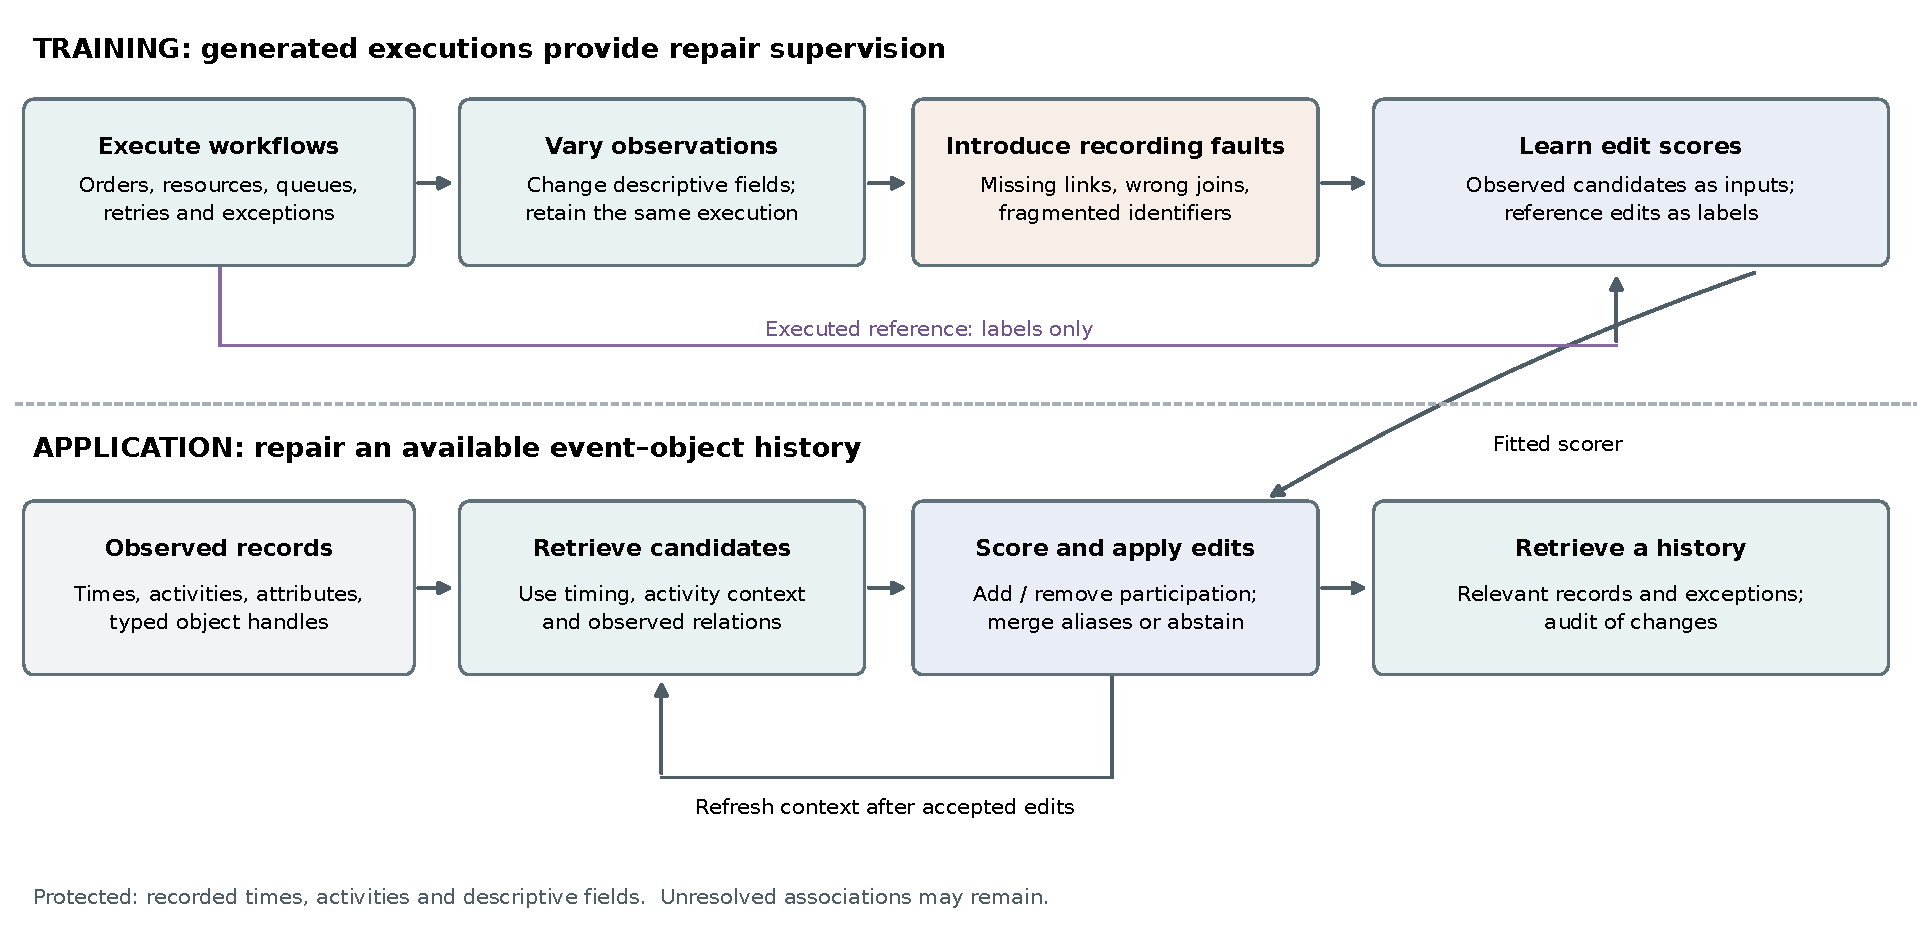
\includegraphics[width=\linewidth]{figures/method_overview.pdf}
\caption{The implemented training and application boundary. Executed references supervise training labels. At application time, candidate retrieval and edit scoring use the observed temporal graph. The system retains recorded event content and can leave uncertain associations unresolved.}
\label{fig:method}
\end{figure}
\subsection{Execution, observation and task construction}
A world executes a finite workflow with parents, work items, resources and optional batches. Mechanisms include branching and joining, resource queues, handoffs, batching, retries, cancellation and return. The expanded configuration adds finite multistage work routes, repeated work, start/completion records and waiting-time variation. Resource-capacity constraints are enforced when queueing is enabled. These are symbolic mechanisms, not a calibrated organizational digital twin.

Observation projection selects visible entity types and descriptive fields before faults are applied. Clean and damaged variants share execution ancestry. The repair task exports a public learner graph and separate reference participation, identity and fault records. A second task exports available prefix observations and future-participation targets from the same execution, excluding future-born entities from the candidate catalog. This reuse is a bounded interface check, not evidence for a universal dataset platform.

Each execution records its normalized recipe, random states, source fingerprint and pending work. A JSON checkpoint resumes to the same execution as an uninterrupted run. Export manifests hash learner, reference and metadata files; observations derived from one execution remain in the same split. Changing source code invalidates incompatible checkpoints.

\subsection{Paired observation generation}
The principal comparison changes descriptive fields while keeping executed events, visible entity types, timestamps and corruption references fixed. Each world receives one of four seeded observation profiles: original fields; activity-dependent categories; numerical measurements; or a mixture of activity categories, measurements, incidental categories and time bands. Fields can be sparse. Numerical measurements combine an existing amount, when available, with activity-dependent scales and noise; no field is derived from a target identifier. Every clean/damaged pair receives the same aligned event descriptions through builder-only execution ancestry. This is an application of observation randomization, not a new general randomization principle.

The comparison holds world count, execution recipes, fault realizations, sampled query events, learner capacity and generated calibration collection fixed within each trial. Observation changes can alter candidate retrieval and therefore the number of unique candidate pairs. It is consequently not an exactly equal number of binary training examples. Independent repetitions regenerate the executed worlds and their observation fields.

\subsection{Variation and held-out conditions}
Training and generated validation use disjoint mechanism compositions. Vocabulary profiles vary independently of flat versus multi-object projection. The profiles share one simulator engine and therefore do not constitute independent domains. History length, resource count, waiting scales, attribute collisions and error severity vary independently within the declared schedule.

The original recording faults combine contiguous or independent missing participation, same-type incorrect joins and time-cut identity fragmentation. An independently implemented development stressor uses activity-routed namespaces, a recording outage over a time interval and persistent stale join mappings. Its rates are declared experimental conditions, not estimates of real incident frequencies. Both fault families preserve recorded activity and time.

\section{Auditable learned graph edits}
Candidate retrieval combines temporal proximity, activity context, observed co-participation and descriptive agreement. Candidate recall is reported separately from classifier performance. Handles are anonymous identifiers, never numerical predictors. Cold objects with no evidence remain difficult or unidentifiable; reference knowledge does not make them recoverable from the learner input.

For participation candidates, the learner uses degree, normalized context overlap, temporal bracketing, activity transitions and attribute agreement. The queried event is excluded from supporting history when assessing its current association. Identity candidates use symmetric history and context features, including overlap, activity profiles, observed attributes and temporal boundary compatibility. Overlapping lifetimes are permitted in candidate retrieval.

Training references label candidate edits and create valid partial-repair states. They are never inputs to the candidate constructor or inference scorer. The boosted control uses separate conditional action classifiers. It is a discriminative edit learner trained with generated supervision, not a deep generative density model. Neural controls use the same candidate action features and graph-derived node inputs, with temporal message passing, relation-specific mean GraphSAGE or no graph messages.

At inference, the system scores candidate edits, selects a commuting batch, applies it and recomputes evidence. A batch cannot merge an entity while also modifying its participation. The implementation records scores and reversible changes. Development thresholds and the pass limit determine abstention; the thresholds do not provide an out-of-domain precision guarantee. One-pass and fixed-sequence variants isolate the benefit of revisiting the graph. Repeated source-trained matching is also a required comparator.

The generated reference labels a merge positive when its handles refer to the same entity, a removal positive when the recorded participant is incorrect, and an addition positive when it supplies a missing reference entity. These are local edit labels, not an optimization guarantee for final history F1. Training also includes partial teacher-repaired states to expose the learner to updated context. At inference, an accepted participation edit cannot subsequently be reversed and an identity merge cannot be split. Although the audit can undo a batch, the learned decoder has no search or backtracking policy; an early mistake can therefore persist.

\section{Evaluation design}
\subsection{Sources and splits}
BPI 2012~\cite{bpi2012} and the public simulated logistics log are development sources. BPI 2012 cases are assigned to fit, tune and reserved check partitions before anonymization. Shared resource types are allowed, but held-out events do not enter another partition's observation context. BPI 2017~\cite{bpi2017} and BPI 2019~\cite{bpi2019} cohorts were reserved until the models, calibration caches, adapters, faults and comparisons were frozen. Their confirmation experiments are now running.

BPI 2017 contains applications and explicitly recorded offers from the same institution as BPI 2012, after a supporting-system change. It does not establish transfer to an unseen organization. We select 1,024 applications by seeded hash rank after excluding the first 500 applications inspected for feasibility and their offers. The resulting cohort contains 38,822 events and 2,422 target entities (1,024 applications and 1,398 offers). Only explicit event-level offer references become offer participation; absence of an offer reference is not a certified absence of a real-world offer relationship.

For BPI 2019 we use the released OCEL conversion~\cite{bpiconversion,bpiocel}, selecting 1,024 purchase orders after excluding orders and items occurring in the first 2,000 feasibility-audited events. The cohort contains 20,396 events and 4,325 target entities (1,024 orders and 3,301 items). Resource and vendor relations remain observed context. Here ``native'' refers to the released OCEL representation, not a claim that every relation was an explicit field in the original XES event. Copied trace attributes, identifier fields and object-to-object relations are removed from learner input. The retained descriptive event field is cumulative net worth. The reserved BPI 2012 check partition contains 42,366 events and 2,034 application histories; its copied requested amount is explicitly labeled as denormalized.

The expanded executable collection contains 512 training worlds and 96 validation worlds. The independent relational/OCEL collection uses BatteryVault and ClaimStream as development domains, selected by alphabetical order before record inspection; its remaining four scenarios are reserved for confirmation. These are external simulations, not additional real-world datasets.

Final experiments must distinguish synthetic-only learning, source-only learning, mixed learning and any target-data adaptation. For limited source annotation, a verified history supplies its event memberships and alias handles. All available annotated positive pairs may train the matcher even if candidate retrieval missed them; inference retrieval remains label-free. Development label budgets must not be described as total annotation costs when additional labeled validation data select thresholds.

\subsection{Application outcomes}
For an observed handle, the predicted cluster returns an event-history set. We compare this set with the reference entity history. Scores are first averaged across handles belonging to the same reference entity and then across entities, preventing heavily fragmented entities from dominating the metric. We report history precision, recall, F1 and the fraction of exactly restored histories. Identity-pair precision and recall expose false merges and unresolved fragments.

Operational queries measure whether a handle retrieves evidence of a cancellation-related event and whether the first and last recorded timestamps are correctly recovered. Matching a boundary timestamp does not imply that every simultaneous boundary event is restored. These queries concern recorded evidence, not a causal judgment that an entire business transaction was canceled. Correct-event preservation, cold-history coverage, genuine exception associations, candidate coverage and runtime accompany aggregate repair scores.

\section{Development evidence and decisions}
Table~\ref{tab:dev} contains exploratory results, not frozen final comparisons. Generated-data thresholds are selected on generated validation. The table is intended to make development decisions auditable while confirmation remains outstanding.

\begin{table}[ht]
\centering
\begin{tabular}{lrr}
\toprule
Expanded generated validation (24 worlds) & Damaged F1 & Clean F1\\
\midrule
No repair & .7429 & 1.0000\\
Boosted edits, one pass & .7996 & .99984\\
MLP edits, iterative & .8243 & .99975\\
Temporal message passing, iterative & .8182 & .99984\\
Heterogeneous GraphSAGE, iterative & .8384 & .99854\\
Boosted edits, fixed sequence & .8500 & .99964\\
Boosted edits, coordinated & .8529 & .99964\\
\bottomrule
\end{tabular}
\caption{Development history F1. Differences between coordinated and fixed-sequence decoding are small; the neural encoder does not improve this collection. Independent confirmation and multiple seeds remain required.}
\label{tab:dev}
\end{table}

On the explored BPI 2012 tune graph with denormalized amount observations, synthetic-only boosted edits raise history F1 from .7445 to .8380. This run uses no real-source training labels and selects its thresholds on generated validation. It preserves 31,101 of 31,362 initially correct event assignments and merges 18 identity pairs, 17 correctly. Its low identity recall (.0479) limits any claim of complete identity restoration.

The source-trained participant matcher reaches .8922 history F1. Adding a learned source identity matcher reaches .9107, and refreshing both matchers reaches .9164 in a second cycle. These stronger controls must remain visible. The synthetic policy is useful in this development setting but does not surpass source supervision. Under the independent pipeline faults on generated validation, history F1 rises only from .7465 to .7811, indicating a substantial recording-mechanism transfer limitation.

The development conclusion is to retain boosted matching as the leading learner, investigate source-label efficiency and recording-mechanism transfer, and avoid presenting the temporal neural architecture as the contribution. Final tables will replace this section only after the declared confirmation protocol is completed.

At a fixed budget of 16 verified source training histories, generated augmentation raises history F1 from .8359 to .8912. At 64 histories, the corresponding values are .8321 and .8905. Both comparisons use additional source-development labels for threshold selection and therefore do not establish total annotation costs of 16 or 64 histories.

At 256 verified training histories, the source-only and augmented results are .8753 and .8896. Augmentation gains are smaller at this budget, and neither sequence is monotonically increasing. These single-seed results motivate repeated, fully budgeted comparisons rather than an unconditional label-efficiency claim.

The first independent-simulator tests expose a failure of the original model. On native event attributes, BatteryVault history F1 decreases from .7682 to .7371, and ClaimStream from .7617 to .7519. Excessive removal of valid associations is a principal observed error. The model's good generated-validation preservation therefore does not establish safe transfer. Structural-only diagnostics and a control trained through additional corruption of already imperfect source observations are being evaluated before revising the method.

The completed attribute-hiding diagnostic raises F1 to .8543 in BatteryVault and .8844 in ClaimStream (Figure~\ref{fig:views}), retaining timing, activities and observed relations. On BatteryVault's clean counterpart, history F1 remains .99945. These development-selected diagnostics do not yet specify a final automatic observation policy. Using evaluator-only native exception flags consistently across views, exception-evidence retrieval F1 improves from .8700 to .9244 for BatteryVault and from .8374 to .9510 for ClaimStream. The first structural diagnostic incorrectly derived its exception-positive set from hidden learner fields; a separate corrected query audit preserves the original history results and uses the pinned native parent records for evaluation labels.

\begin{figure}[ht]
\centering
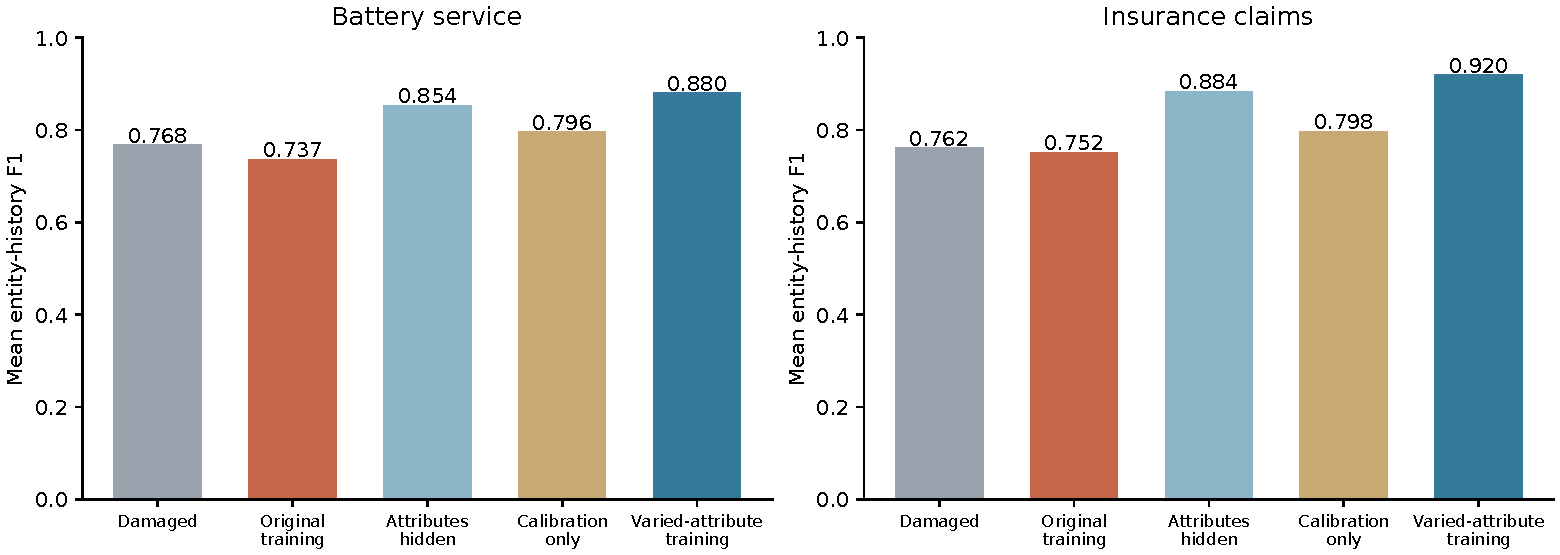
\includegraphics[width=\linewidth]{figures/development_observation_views.pdf}
\caption{Single-run development comparison on the same independent-simulator records and faults. Original training fails with native fields. Hiding attributes is a manual diagnostic; calibration-only retains the original fitted model. Varied-attribute training changes generated observations while preserving the executed workflows and fault labels. All operating points use generated validation.}
\label{fig:views}
\end{figure}

The paired observation-generation revision improves native-field history F1 to .8804 on BatteryVault and .9197 on ClaimStream. Keeping the original model but changing its generated calibration reaches only .7964 and .7978, separating a training-data benefit from a calibration-only effect. The revised model makes zero changes on the clean counterparts of both domains. Under mixed faults, it preserves 17,624 of 17,708 and 18,267 of 18,325 initially correct events. Exception-evidence F1 reaches .9247 and .9648. Identity recall remains incomplete: 69 of 246 and 199 of 403 true identity pairs are restored, with nine and four incorrect predicted pairs.

This revision has a measured trade-off: BPI 2012 tune history F1 decreases from .8380 with the original generated learner to .8074. An alternative automatic field-stability filter reaches .8393 on BPI and .8588/.8920 on the two independent simulations. The filter keeps fields whose observed within-entity agreement exceeds chance-adjusted between-entity agreement by the development threshold .5. Neither approach dominates across all three development sources. A final claim must therefore report per-process outcomes and retain this negative comparison.

Using the same original generated calibration, a control trained only to undo extra corruption of imperfect BPI observations reaches .7551 history F1. Combining that noisy pseudo supervision with generated training reaches .8329, compared with .8380 for generated training alone. Target-local versions of this control, independently repeated world collections and refitted scoring-feature ablations remain in progress at this draft stage.

\section{Limitations and outstanding validation}
The workflows share one symbolic implementation; vocabulary changes are not independent domains. Generated behavior is not calibrated to any particular company. Public-source corruption tests do not establish effectiveness on naturally occurring, independently labeled errors. The task assumes an entity catalog, protected event fields and offline context. Some object identities are observationally indistinguishable, so exact recovery is impossible without additional evidence.

Current results use development-selected operating points and mostly one training seed. A few positive labels can make identity calibration abstain entirely. Generated-data gains may depend on training volume, history-length coverage and observation attributes; matched-budget ablations are needed to separate those factors. The final package must include source hashes, command manifests, split definitions, data permissions, uncertainty across repeated runs, failure cases, code and model artifacts, and a critical claim-by-claim review. No acceptance outcome is guaranteed by the current draft.

\appendix
\section{Implementation details}
The principal learner fits one histogram gradient-boosting classifier per edit operation, with 200 boosting iterations, at most 15 leaves, learning rate .08 and $L_2$ regularization 1. Early stopping is disabled and the fitting seed is zero. Positive and negative examples each receive half the aggregate training weight. This fixed learner isolates the effect of generated observations; it is not proposed as a new learning architecture.

Participation scoring uses 18 history-matching features plus observed type/activity prevalence and same-type event degree. Identity scoring uses 25 symmetric history-matching features. These are placed in a shared 28-dimensional action vector and clipped to $[-10,10]$. Retrieval and feature construction exclude the queried event from its supporting history. Training samples up to 48 events per state, 16 participation candidates per event/type and 32 identity candidates per handle. Candidate generation never receives the reference labels. The 512-world training collection supplies 896 states: 512 damaged states, 128 clean states and 256 partial-repair states. Generated validation supplies 120 states from 96 worlds.

For each operation, the threshold maximizes empirical recall among generated-validation thresholds with empirical precision at least .95 and at least five true positives. If none meets this criterion, that operation abstains. Scores from class-weighted training are not asserted to be calibrated probabilities. Threshold selection is a finite validation rule, with no statistical precision guarantee on a new process. The real-source and independent-simulator protocol permits four passes with participation/pair budgets 128/64; the generated compositional test uses eight passes and budgets 16/32. Thus the two test regimes are reported separately.

Neural controls use width 64, two message-passing layers where applicable, 16-dimensional node features, type/activity embeddings and three edit heads. GraphSAGE uses a root projection and relation-specific mean-neighbor projections. Its adjacency includes event--object incidence and temporal neighbor relations; removing numerical edge-time inputs does not make it a time-free model. The temporal control additionally uses signed relative-time edge features and learned message gates. The MLP omits message passing but retains shared temporal node/action inputs. All three controls use the same precomputed candidate universe and generated collections. Neural training samples at most 2,048 actions per state, including at most half positives; boosted training uses all cached candidates. This optimization-budget difference limits architectural conclusions.

The revised neural controls train for 16 epochs with AdamW (learning rate .001, weight decay .0001), cosine decay to .0001, gradient clipping at 5 and dropout .1. The mean generated-validation average precision across operations selects the checkpoint; epoch 10 was selected for all three revised controls. Positive loss weights are computed from training frequencies and capped at 30. No reserved-target labels select checkpoints or thresholds.

\section{Illustrative application audit}
Figure~\ref{fig:cases} shows two post hoc examples from BatteryVault development. The success case is an exception-bearing history whose improvement is nearest the median positive improvement among such histories. The failure case has the largest history-F1 loss. Ties use a hash of the opaque identifier. These illustrations explain behavior and are not separate evidence of generalization.
\begin{figure}[ht]
\centering
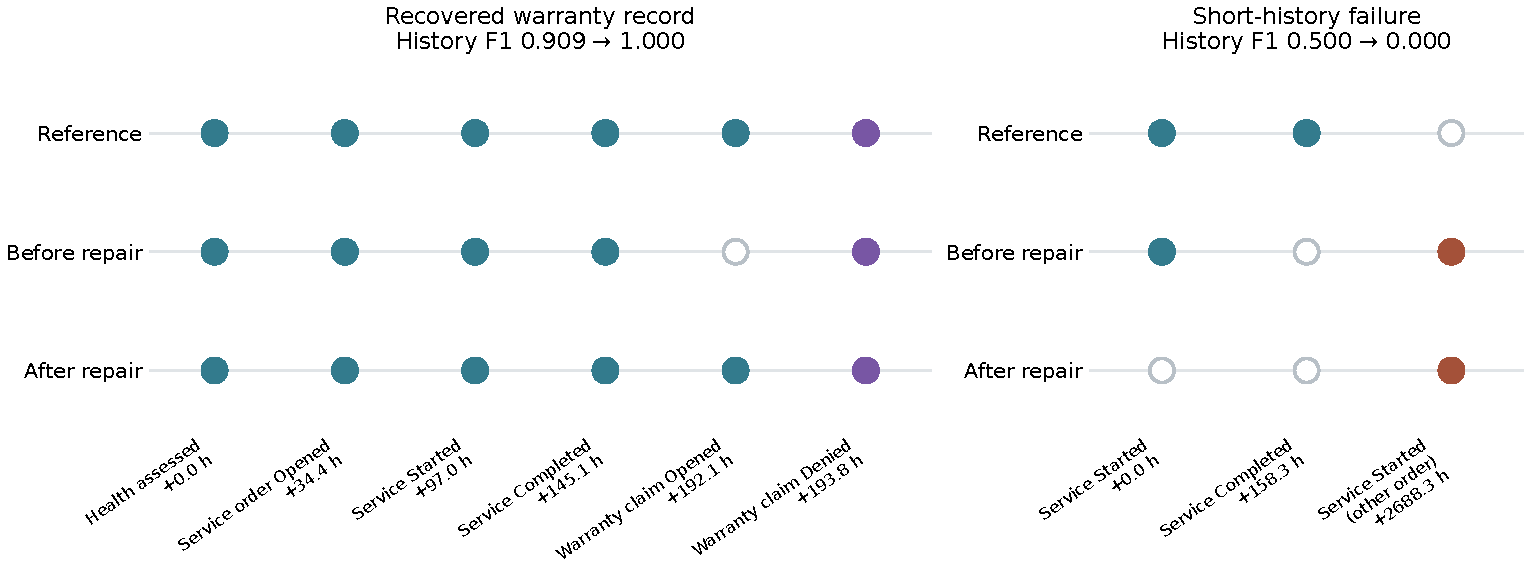
\includegraphics[width=\linewidth]{figures/development_application_cases.pdf}
\caption{A recovered warranty record and a failed short service history. Filled circles are retrieved records; empty circles are absent. Purple denotes a genuine exception, and rust a record belonging to another order. Times are relative to the first displayed record, with chronological but evenly spaced columns. Entity scores average over aliases; the diagram displays one hash-selected handle.}
\label{fig:cases}
\end{figure}

\begin{thebibliography}{99}
\bibitem{here} F. Zetzsche et al. \emph{Case ID Revealed HERE: Hybrid Elusive Case Repair Method for Transformer-Driven Business Process Event Log Enhancement}. Business \& Information Systems Engineering 67, 311--337, 2025. \url{https://doi.org/10.1007/s12599-025-00935-5}.
\bibitem{sanagraph} S. Dissegna, C. Di Francescomarino and M. Ronzani. \emph{Graph-Based Event Log Repair}. CAiSE 2026, 423--440. \url{https://doi.org/10.1007/978-3-032-28117-3_24}. Accessible author preprint: \url{https://arxiv.org/abs/2508.05145}.
\bibitem{ddtr} M. Matyash, A. Gal and A. Senderovich. \emph{DDTR: Diffusion Denoising Trace Recovery}. 2025. \url{https://arxiv.org/abs/2510.22553}.
\bibitem{holoclean} T. Rekatsinas, X. Chu, I. F. Ilyas and C. R\'e. \emph{HoloClean: Holistic Data Repairs with Probabilistic Inference}. 2017. \url{https://arxiv.org/abs/1702.00820}.
\bibitem{ocsim} B. Knopp, M. Pourbafrani and W. M. P. van der Aalst. \emph{Discovering Object-Centric Process Simulation Models}. ICPM 2023. \url{https://ieeexplore.ieee.org/document/10271944/}.
\bibitem{relationalocel} A. Berti. \emph{Synthetic relational databases and reference OCELs}. Zenodo, version 1, 2026. \url{https://doi.org/10.5281/zenodo.22079246}.
\bibitem{ekginference} A. Swevels, R. Dijkman and D. Fahland. \emph{Inferring Missing Entity Identifiers from Context Using Event Knowledge Graphs}. BPM 2023, 180--197. \url{https://doi.org/10.1007/978-3-031-41620-0_11}.
\bibitem{ocip} S. Sadeghianasl et al. \emph{Object-centric event-data imperfection patterns}. Information Systems 141, 102766, 2026. \url{https://doi.org/10.1016/j.is.2026.102766}.
\bibitem{flawd} M. Comuzzi, J. Ko and F. M. Maggi. \emph{A Language to Model and Simulate Data Quality Issues in Process Mining}. ACM J. Data Inf. Qual. 17(2), Article 6, 2025. \url{https://doi.org/10.1145/3743144}.
\bibitem{repairlanguage} S. Sadeghianasl, R. Dijkman, R. Andrews and A. Barros. \emph{A Language for Efficient Event Log Repair}. EDOC 2026. Conference record: \url{https://conf.researchr.org/details/edoc-2026/edoc-2026-papers/8/A-Language-for-Efficient-Event-Log-Repair}.
\bibitem{domainrandomization} J. Tobin, R. Fong, A. Ray, J. Schneider, W. Zaremba and P. Abbeel. \emph{Domain Randomization for Transferring Deep Neural Networks from Simulation to the Real World}. 2017. \url{https://arxiv.org/abs/1703.06907}.
\bibitem{plurel} V. Kothapalli, R. Ranjan, V. Hudovernik, V. P. Dwivedi, J. Hoffart, C. Guestrin and J. Leskovec. \emph{PluRel: Synthetic Data unlocks Scaling Laws for Relational Foundation Models}. 2026. \url{https://arxiv.org/abs/2602.04029}.
\bibitem{rdbpfn} Y. Wang, J. You, C. Shi and M. Zhang. \emph{Relational In-Context Learning via Synthetic Pre-training with Structural Prior}. 2026. \url{https://arxiv.org/abs/2603.03805}.
\bibitem{tigger} S. Gupta, S. Manchanda, S. Bedathur and S. Ranu. \emph{TIGGER: Scalable Generative Modelling for Temporal Interaction Graphs}. AAAI 36(6), 6819--6828, 2022. \url{https://doi.org/10.1609/aaai.v36i6.20638}.
\bibitem{bpi2012} B. F. van Dongen. \emph{BPI Challenge 2012}. Dataset, 2012. \url{https://doi.org/10.4121/uuid:3926db30-f712-4394-aebc-75976070e91f}.
\bibitem{bpi2017} B. F. van Dongen. \emph{BPI Challenge 2017}. Dataset, 2017. \url{https://doi.org/10.4121/uuid:5f3067df-f10b-45da-b98b-86ae4c7a310b}.
\bibitem{bpi2019} B. F. van Dongen. \emph{BPI Challenge 2019}. Dataset, 2019. \url{https://doi.org/10.4121/uuid:d06aff4b-79f0-45e6-8ec8-e19730c248f1}.
\bibitem{bpiconversion} S. Khayatbashi, O. Hartig and A. Jalali. \emph{Transforming Event Knowledge Graph to Object-Centric Event Logs: A Comparative Study for Multi-dimensional Process Analysis}. ER 2023, 220--238. \url{https://doi.org/10.1007/978-3-031-47262-6_12}.
\bibitem{bpiocel} S. Khayatbashi and A. Jalali. \emph{BPI Challenge datasets---OCEL 2.0}. Zenodo, version 1, 2026. \url{https://doi.org/10.5281/zenodo.22663565}.
\end{thebibliography}
\end{document}
